\documentclass[border=6pt]{standalone}
\usepackage[T1]{fontenc}
\usepackage{courier}
\usepackage[scaled=0.95]{helvet}
\renewcommand{\familydefault}{\sfdefault}
\usepackage{sfmath}
\usepackage[version=4]{mhchem}
\usepackage{tikz}
\usepackage{pgfplots}
\pgfplotsset{compat=newest}
\usetikzlibrary{arrows.meta,positioning,calc,fit,backgrounds,shapes.geometric,decorations.pathreplacing,patterns}
\definecolor{ink}{HTML}{17233A}
\definecolor{inksoft}{HTML}{44506A}
\definecolor{teal}{HTML}{0E6B6B}
\definecolor{tealsoft}{HTML}{E5F0EF}
\definecolor{amber}{HTML}{B26B12}
\definecolor{ambersoft}{HTML}{FBF0DF}
\definecolor{blue}{HTML}{2F6690}
\definecolor{bluesoft}{HTML}{E3ECF4}
\definecolor{plum}{HTML}{7A4D8C}
\definecolor{plumsoft}{HTML}{EFE7F3}
\definecolor{greyc}{HTML}{8A94A3}
\definecolor{linec}{HTML}{D3DCE1}
\definecolor{oxy}{HTML}{C0392B}
\definecolor{carb}{HTML}{3B4252}
\definecolor{hyd}{HTML}{E6E9EE}
\definecolor{nit}{HTML}{2F6690}
\tikzset{
  every picture/.style={line cap=round,line join=round},
  lab/.style={font=\small, text=inksoft},
  >={Stealth[length=7pt]},
}
\pgfplotsset{
  every axis/.append style={axis line style={inksoft}, tick style={inksoft}, tick label style={font=\footnotesize, text=inksoft}, label style={font=\small, text=ink}},
}
% fragment tile: \frag{node name}{position}{colour}{content}
\newcommand{\frag}[4]{\node[draw=#3, fill=#3!12, line width=1.4pt, rounded corners=6pt, minimum width=1.25cm, minimum height=1.05cm, text=#3, font=\bfseries] (#1) at (#2) {#4};}
\newcommand{\ring}{\tikz[baseline=-0.6ex]{\draw[line width=1.1pt] (0:0.3)--(60:0.3)--(120:0.3)--(180:0.3)--(240:0.3)--(300:0.3)--cycle; \draw[line width=0.8pt] (0,0) circle (0.16);}}
\newcommand{\bond}[2]{\draw[ink, line width=2.2pt] (#1) -- (#2);}

\begin{document}
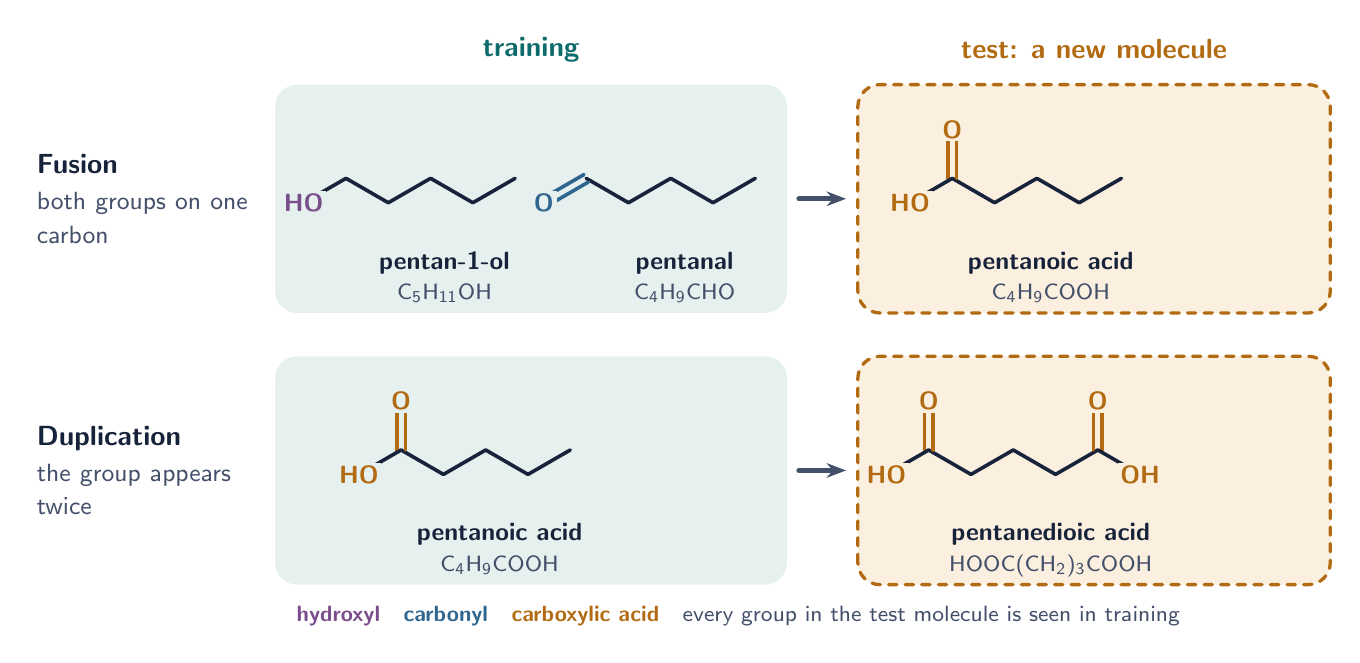
\begin{tikzpicture}
\node[font=\bfseries, text=teal] at (6.4,3.75) {training};
\node[font=\bfseries, text=amber] at (13.55,3.75) {test: a new molecule};
\node[anchor=west, align=left, text width=2.9cm] at (0,1.85) {\textbf{\textcolor{ink}{Fusion}}\\[1pt]{\small\color{inksoft}both groups on one carbon}};
\fill[tealsoft, rounded corners=8pt] (3.15,0.40) rectangle (9.65,3.30);
\draw[amber, dashed, line width=1.2pt, fill=ambersoft, rounded corners=8pt] (10.55,0.40) rectangle (16.55,3.30);
\draw[->, inksoft, line width=1.7pt] (9.8,1.85) -- (10.4,1.85);
\draw[ink, line width=1.3pt] (4.050,2.110) -- (4.587,1.800);
\draw[ink, line width=1.3pt] (4.587,1.800) -- (5.124,2.110);
\draw[ink, line width=1.3pt] (5.124,2.110) -- (5.661,1.800);
\draw[ink, line width=1.3pt] (5.661,1.800) -- (6.198,2.110);
\draw[ink, line width=1.3pt] (4.050,2.110) -- (3.513,1.800);
\node[font=\small\bfseries, text=plum, fill=tealsoft, inner sep=1pt, anchor=center] at (3.513,1.800) {HO};
\node[align=center, anchor=north] at (5.30,1.30) {{\small\bfseries\color{ink}pentan-1-ol}\\[-1pt]{\footnotesize\color{inksoft}\ce{C5H11OH}}};
\draw[ink, line width=1.3pt] (7.100,2.110) -- (7.637,1.800);
\draw[ink, line width=1.3pt] (7.637,1.800) -- (8.174,2.110);
\draw[ink, line width=1.3pt] (8.174,2.110) -- (8.711,1.800);
\draw[ink, line width=1.3pt] (8.711,1.800) -- (9.248,2.110);
\draw[blue, line width=1.3pt] (7.127,2.062) -- (6.591,1.752);\draw[blue, line width=1.3pt] (7.072,2.158) -- (6.536,1.848);
\node[font=\small\bfseries, text=blue, fill=tealsoft, inner sep=1pt, anchor=center] at (6.563,1.800) {O};
\node[align=center, anchor=north] at (8.35,1.30) {{\small\bfseries\color{ink}pentanal}\\[-1pt]{\footnotesize\color{inksoft}\ce{C4H9CHO}}};
\draw[ink, line width=1.3pt] (11.750,2.110) -- (12.287,1.800);
\draw[ink, line width=1.3pt] (12.287,1.800) -- (12.824,2.110);
\draw[ink, line width=1.3pt] (12.824,2.110) -- (13.361,1.800);
\draw[ink, line width=1.3pt] (13.361,1.800) -- (13.898,2.110);
\draw[amber, line width=1.3pt] (11.695,2.110) -- (11.695,2.730);\draw[amber, line width=1.3pt] (11.805,2.110) -- (11.805,2.730);
\node[font=\small\bfseries, text=amber, fill=ambersoft, inner sep=1pt, anchor=center] at (11.750,2.730) {O};
\draw[ink, line width=1.3pt] (11.750,2.110) -- (11.213,1.800);
\node[font=\small\bfseries, text=amber, fill=ambersoft, inner sep=1pt, anchor=center] at (11.213,1.800) {HO};
\node[align=center, anchor=north] at (13.00,1.30) {{\small\bfseries\color{ink}pentanoic acid}\\[-1pt]{\footnotesize\color{inksoft}\ce{C4H9COOH}}};
\node[anchor=west, align=left, text width=2.9cm] at (0,-1.60) {\textbf{\textcolor{ink}{Duplication}}\\[1pt]{\small\color{inksoft}the group appears twice}};
\fill[tealsoft, rounded corners=8pt] (3.15,-3.05) rectangle (9.65,-0.15);
\draw[amber, dashed, line width=1.2pt, fill=ambersoft, rounded corners=8pt] (10.55,-3.05) rectangle (16.55,-0.15);
\draw[->, inksoft, line width=1.7pt] (9.8,-1.60) -- (10.4,-1.60);
\draw[ink, line width=1.3pt] (4.750,-1.340) -- (5.287,-1.650);
\draw[ink, line width=1.3pt] (5.287,-1.650) -- (5.824,-1.340);
\draw[ink, line width=1.3pt] (5.824,-1.340) -- (6.361,-1.650);
\draw[ink, line width=1.3pt] (6.361,-1.650) -- (6.898,-1.340);
\draw[amber, line width=1.3pt] (4.695,-1.340) -- (4.695,-0.720);\draw[amber, line width=1.3pt] (4.805,-1.340) -- (4.805,-0.720);
\node[font=\small\bfseries, text=amber, fill=tealsoft, inner sep=1pt, anchor=center] at (4.750,-0.720) {O};
\draw[ink, line width=1.3pt] (4.750,-1.340) -- (4.213,-1.650);
\node[font=\small\bfseries, text=amber, fill=tealsoft, inner sep=1pt, anchor=center] at (4.213,-1.650) {HO};
\node[align=center, anchor=north] at (6.00,-2.15) {{\small\bfseries\color{ink}pentanoic acid}\\[-1pt]{\footnotesize\color{inksoft}\ce{C4H9COOH}}};
\draw[ink, line width=1.3pt] (11.450,-1.340) -- (11.987,-1.650);
\draw[ink, line width=1.3pt] (11.987,-1.650) -- (12.524,-1.340);
\draw[ink, line width=1.3pt] (12.524,-1.340) -- (13.061,-1.650);
\draw[ink, line width=1.3pt] (13.061,-1.650) -- (13.598,-1.340);
\draw[amber, line width=1.3pt] (11.395,-1.340) -- (11.395,-0.720);\draw[amber, line width=1.3pt] (11.505,-1.340) -- (11.505,-0.720);
\node[font=\small\bfseries, text=amber, fill=ambersoft, inner sep=1pt, anchor=center] at (11.450,-0.720) {O};
\draw[ink, line width=1.3pt] (11.450,-1.340) -- (10.913,-1.650);
\node[font=\small\bfseries, text=amber, fill=ambersoft, inner sep=1pt, anchor=center] at (10.913,-1.650) {HO};
\draw[amber, line width=1.3pt] (13.543,-1.340) -- (13.543,-0.720);\draw[amber, line width=1.3pt] (13.653,-1.340) -- (13.653,-0.720);
\node[font=\small\bfseries, text=amber, fill=ambersoft, inner sep=1pt, anchor=center] at (13.598,-0.720) {O};
\draw[ink, line width=1.3pt] (13.598,-1.340) -- (14.135,-1.650);
\node[font=\small\bfseries, text=amber, fill=ambersoft, inner sep=1pt, anchor=center] at (14.135,-1.650) {OH};
\node[align=center, anchor=north] at (13.00,-2.15) {{\small\bfseries\color{ink}pentanedioic acid}\\[-1pt]{\footnotesize\color{inksoft}\ce{HOOC(CH2)3COOH}}};
\node[font=\footnotesize, text=inksoft, anchor=west] at (3.3,-3.45) {\textcolor{plum}{\textbf{hydroxyl}}\quad \textcolor{blue}{\textbf{carbonyl}}\quad \textcolor{amber}{\textbf{carboxylic acid}}\quad every group in the test molecule is seen in training};
\end{tikzpicture}
\end{document}
